% Compile: pdflatex architecture && (optional) included from main.tex
\documentclass[tikz,border=2pt]{standalone}
\usepackage{tikz}
\usetikzlibrary{arrows.meta,positioning,fit,shapes.geometric,calc}

\begin{document}
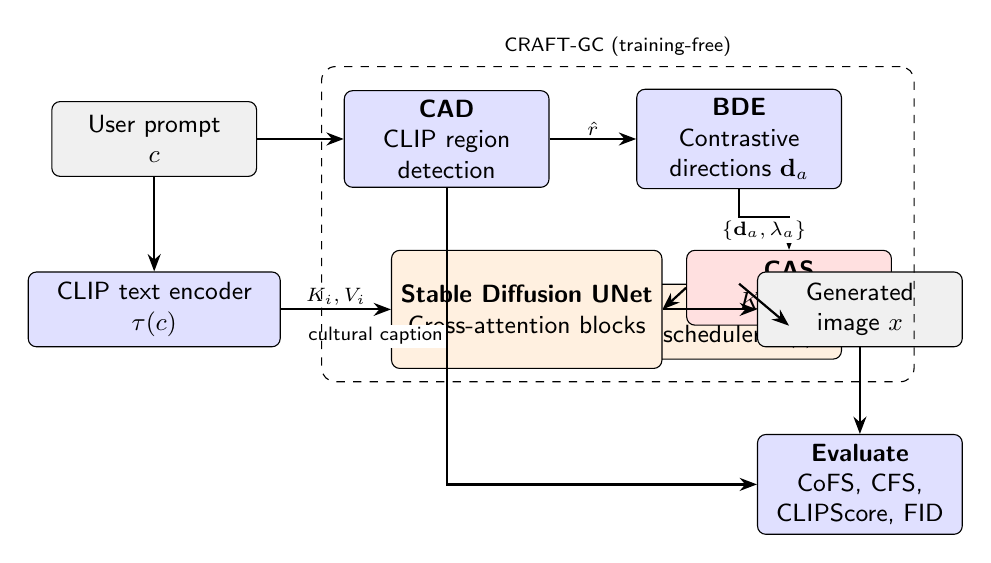
\begin{tikzpicture}[
  font=\small\sffamily,
  box/.style={draw, rounded corners=3pt, align=center, minimum width=2.6cm, minimum height=0.95cm, fill=#1!12},
  module/.style={box=blue},
  data/.style={box=gray},
  proc/.style={box=orange},
  arr/.style={-{Stealth[length=2.2mm]}, thick},
  lbl/.style={font=\scriptsize\sffamily, fill=white, inner sep=1pt}
]

\node[data] (prompt) {User prompt\\$c$};
\node[module, right=1.1cm of prompt] (cad) {\textbf{CAD}\\CLIP region\\detection};
\node[module, right=1.1cm of cad] (bde) {\textbf{BDE}\\Contrastive\\directions $\mathbf{d}_a$};
\node[proc, below=1.2cm of bde] (sched) {\textbf{Timestep}\\scheduler $\beta(t)$};

\node[module, below=1.2cm of prompt, minimum width=3.2cm] (clip) {CLIP text encoder\\$\tau(c)$};
\node[proc, right=1.4cm of clip, minimum width=3.4cm, minimum height=1.5cm] (unet) {\textbf{Stable Diffusion UNet}\\Cross-attention blocks};
\node[module, right=0.3cm of unet.north east, anchor=north west, fill=red!12] (cas) {\textbf{CAS}\\$K_i \rightarrow K_i'$};

\node[data, right=1.2cm of unet] (img) {Generated\\image $x$};
\node[module, below=1.1cm of img] (eval) {\textbf{Evaluate}\\CoFS, CFS,\\CLIPScore, FID};

\draw[arr] (prompt) -- (cad);
\draw[arr] (cad) -- node[lbl, above] {$\hat{r}$} (bde);
\draw[arr] (bde.south) -- ++(0,-0.35) -| node[lbl, near start, below] {$\{\mathbf{d}_a,\lambda_a\}$} (cas.north);
\draw[arr] (sched.north) -- (cas.south);
\draw[arr] (prompt.south) -- (clip.north);
\draw[arr] (clip.east) -- node[lbl, above] {$K_i, V_i$} (unet.west);
\draw[arr] (cas.west) -- (unet.east);
\draw[arr] (unet.east) -- (img.west);
\draw[arr] (img.south) -- (eval.north);
\draw[arr] (cad.south) |- node[lbl, near start, left] {cultural caption} (eval.west);

\node[draw, dashed, rounded corners=5pt, inner sep=8pt, fit=(cad)(bde)(cas)(sched),
  label={[font=\scriptsize\sffamily]above:CRAFT-GC (training-free)}] {};

\end{tikzpicture}
\end{document}
